% 图 10.1 —— 手工重建（5 列点阵 + 上行箭头 + 一条穿行曲线 + 两轴）
%
% ══ 按用户意见重做，原稿是 `emit_hand.py` 自动稿，问题三处 ══
%   ① b₀ 的下标写成 9、a₀ 的下标也写成 9（各一处）
%   ② 箭头**完全没还原**：原稿把每支箭头拆成「杆 + 两根倒钩」共 3~4 段碎线，
%      56 行碎线段拼出来的是圆疙瘩。这里换成单条 `-{Triangle[..]}`。
%   ③ 画面上多了 3 个游离的 `(` `)` 字形 —— probe 把**箭头的墨迹**当成括号认了
%      （框 (162,284,15,60)/(163,393,13,58) 正好是一支竖箭头的形状）。已删。
%
% 参数来源：原书 600dpi 裁切 `src_hi/10.1.png`（1642×1137），逐列扫描实测。
%   标定：y 轴在 px 列 90、x 轴在 px 行 1034；
%         圆点列 px 292/490/678/872/1062/1248/1438 ↔ 画布 169.2/277.0/380.4/485.5/589.8/692.0/795.0
%         ⇒ **1 画布单位 = 1.8313 px**（两路独立标定相差 0.1%）。
%   圆点：5 行，行距 ≈108，与原稿 dots 逐个吻合 —— 不动。
%   箭头（实测，画布单位）：
%     · 每支从「下方圆点上方 21」到「再往上 58.5」，即 (x, 点y-21) → (x, 点y-79.5)
%     · 头：长 20.2、宽 12.6（逐行量墨段：py 503 宽 2 → py 540 宽 23）
%     · 杆宽 3.8
%     · **顶上的点上方也有一支**，但只有列 2/5/7 有（列 1 的那支在画布外、
%       列 3/4/6 实测确实没有）—— 这是原图的不对称，照实画。
\documentclass[12pt]{standalone}
\usepackage{fontspec}
\setsansfont{Arial}
\newfontfamily\mfallback{DejaVu Sans}
\usepackage{tikz}
\usetikzlibrary{arrows.meta}
\begin{document}
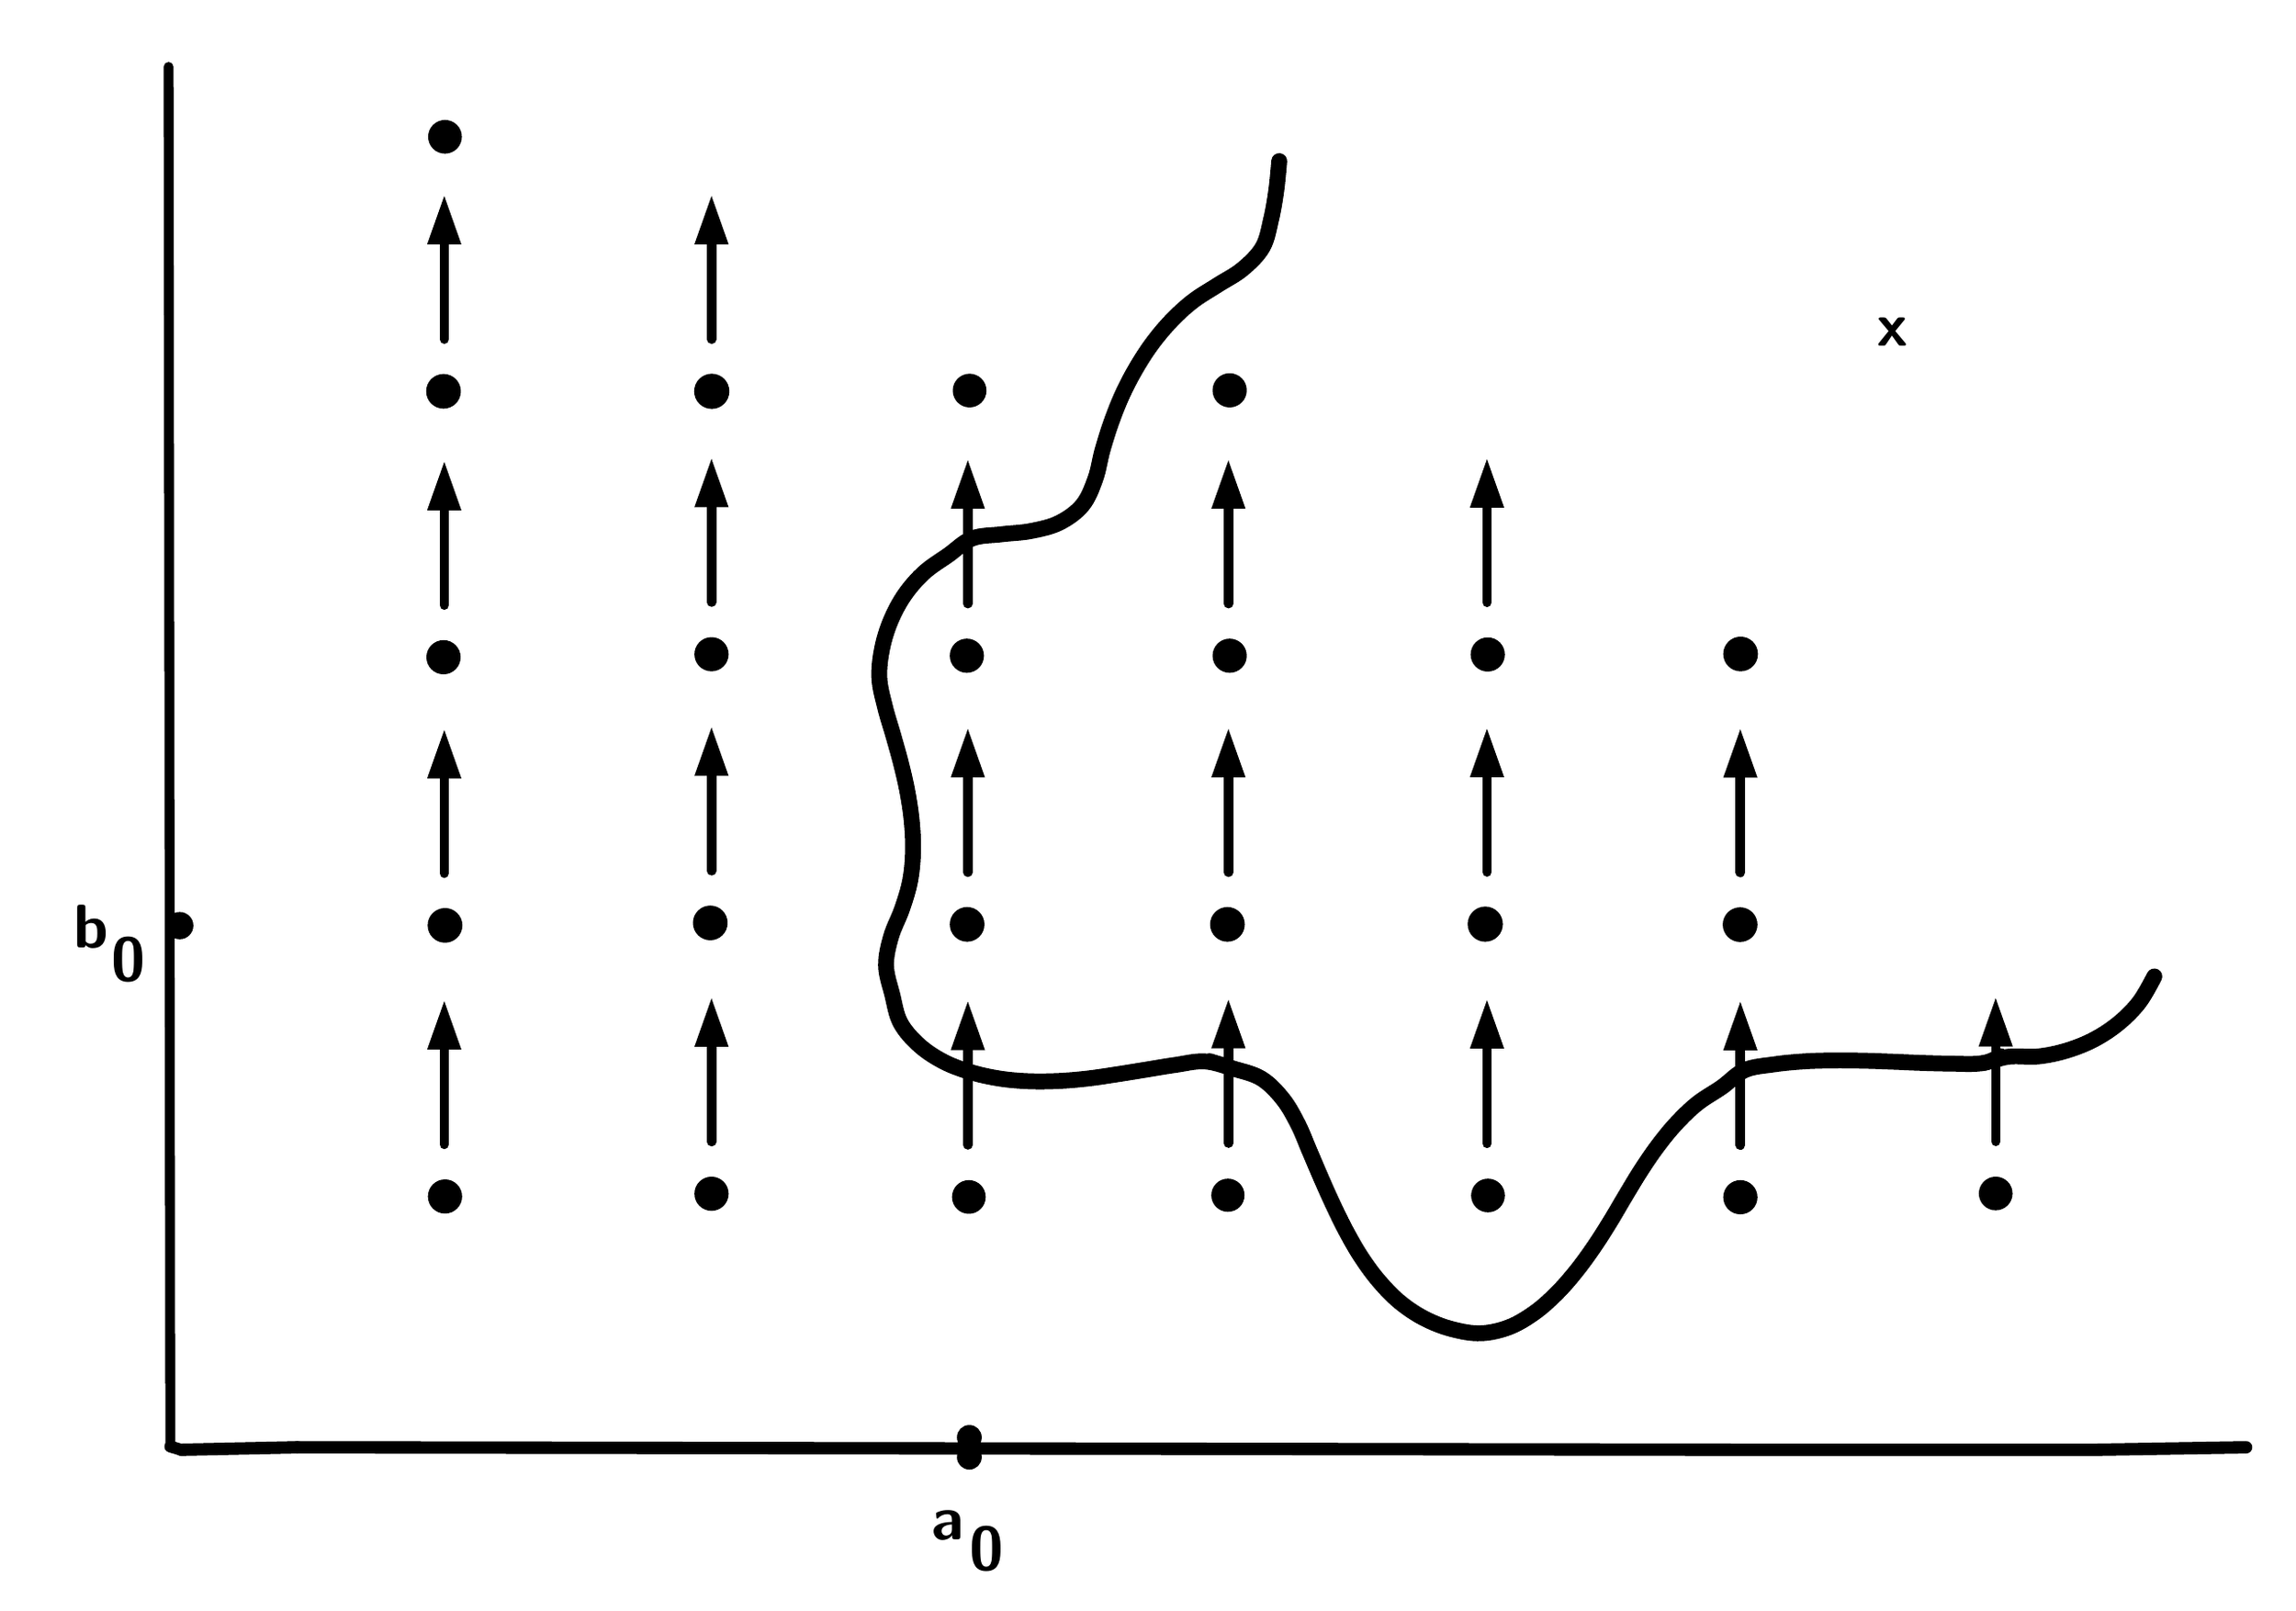
\begin{tikzpicture}[x=1pt, y=-1pt, line width=4.0pt, line cap=round, line join=round]

  %% ════ 两轴 ════
  \draw[line width=4.0pt] (58.0,17.0) -- (58.7,573.7);
  \draw[line width=4.8pt] (58.7,573.7) -- (63.1,575.0);
  \draw[line width=5.0pt] (63.1,575.0) -- (109.9,574.0);
  \draw[line width=5.0pt] (109.9,574.0) -- (694.9,575.0);
  \draw[line width=5.0pt] (694.9,575.0) -- (835.4,575.0);
  \draw[line width=5.0pt] (835.4,575.0) -- (896.0,574.0);

  %% ⚠ 断口搭线：原稿逐段描摹，链上这 3 处端点差 6~9 单位 ⇒ 画出来是断的。
  %%   只补这几小节直线，**不改动原段的坐标与线宽**。
  \draw[line width=6.0pt] (797.0,416.0) -- (790.8,419.0);
  \draw[line width=6.0pt] (487.0,421.0) -- (478.0,418.0);
  \draw[line width=4.0pt] (379.0,211.0) -- (382.0,207.0);
  %% ⚠ 这 3 段原来混在「曲线」里，其实都是**老稿箭头的残段**
  %%   （列 692 的箭杆与箭头、列 380 的箭头、列 485.5 的左侧倒钩）
  %%   ⚠ 上一轮判据用 ±6 漏掉了倒钩（它对列 485.5 偏 7.6）—— 已放宽到 ±9 重审全块。。它们和现在的干净箭头在同一列上叠着，
  %%   在交点处叠出一个台阶/粗疙瘩（用户圈出来的就是这里）。判据：
  %%   一段的**所有点**都落在同一列 x 的 ±6 内 ⇒ 是箭头残段，不是曲线。已删。
  %% ════ 曲线（贯穿全图的折线；原稿的 prims2 curves + 几段落在 strokes 里的）════
  %% ── 贯穿曲线：原稿是 prims2 拆的 **17 段折线链**，实测 —
  %%   · 4 处**断口**：5.0 / 5.0 / 9.5 / 6.9 画布单位
  %%   · 接点**折角** 16.6° ~ 25.5°
  %%   两者叠一起就是用户说的「毛刺」。现按路径采样 -> 补断口 -> 拉普拉斯平滑
  %%   -> 弧长等距重采样，输出**一条** plot[smooth]；端点 (506,55)/(859,384) 与走向不变。
  %%   线宽：原稿有 3 段写 7.0（提取噪声）；在**近竖直段**做水平剖实测原书墨宽
  %%   6.07 / 6.62 / 6.62（横切竖直笔画 = 真线宽），故取 **6.4**（原先写 6.0 偏细）。
  \draw[line width=6.4pt, line cap=round] plot[smooth, tension=0.6] coordinates {
    (506.0,55.0) (504.8,66.9) (502.7,78.6) (499.3,89.8) (491.2,98.6) (481.2,105.0)
    (471.2,111.5) (462.4,119.5) (454.7,128.7) (448.2,138.7) (442.7,149.3) (438.3,160.3)
    (434.7,171.7) (431.8,183.3) (426.6,193.9) (417.2,201.0) (405.7,204.3) (393.9,205.6)
    (382.1,207.3) (372.5,214.0) (362.8,221.0) (355.0,229.9) (349.3,240.4) (345.8,251.8)
    (344.7,263.6) (347.0,275.3) (350.3,286.7) (353.5,298.3) (356.1,309.9) (357.8,321.7)
    (358.3,333.6) (357.1,345.5) (353.8,356.9) (349.4,368.0) (347.4,379.6) (349.9,391.3)
    (353.2,402.7) (360.8,411.8) (370.6,418.4) (381.5,422.6) (393.1,425.2) (405.0,426.3)
    (416.9,426.2) (428.8,425.2) (440.6,423.5) (452.4,421.6) (464.2,419.7) (476.0,418.3)
    (487.5,421.2) (498.8,425.2) (507.4,433.4) (513.5,443.5) (518.2,454.4) (522.9,465.4)
    (527.8,476.3) (533.1,487.0) (539.1,497.3) (546.2,506.9) (554.6,515.4) (564.5,522.0)
    (575.6,526.3) (587.3,528.0) (598.8,525.5) (609.1,519.6) (618.1,511.7) (625.9,502.8)
    (633.0,493.1) (639.4,483.1) (645.5,472.8) (651.7,462.6) (658.4,452.8) (666.0,443.5)
    (674.6,435.3) (684.5,428.7) (693.8,421.8) (705.5,419.5) (717.4,418.3) (729.3,417.9)
    (741.2,418.0) (753.2,418.4) (765.1,418.9) (777.0,419.2) (788.9,419.1) (800.2,416.4)
    (812.1,416.3) (823.7,413.9) (834.8,409.4) (844.7,402.8) (853.0,394.3) (859.0,384.0)};

  %% ════ 箭头 ════
  %% 每支：从 (列x, 该点y-21) 向上画 58.5，头在顶端。
  %% 原稿是 56 行碎线段（杆+两根倒钩分开画），拼出来的头是圆疙瘩。
  \foreach \x/\ty in {%
      169.2/126.9, 169.2/234.2, 169.2/342.4, 169.2/451.8,
      277.0/126.9, 277.0/233.0, 277.0/341.4, 277.0/450.7,
      380.4/233.6, 380.4/342.0, 380.4/452.0,
      485.5/233.6, 485.5/342.0, 485.5/451.3,
      589.8/233.1, 589.8/341.9, 589.8/451.4,
      692.0/342.1, 692.0/452.1,
      795.0/450.6}{
    % ⚠ 单独加 line join=miter：全局是 round，圆角连接会把三角头的
    %   外轮廓描圆，尖端鼓出一小坨（用户指出）。图 7.1 用的就是 miter。
    \draw[line width=3.8pt,line join=miter,
          -{Triangle[width=12.6pt,length=20.2pt]}]
      (\x,\ty) -- (\x,\ty-58.5);
  }

  %% ════ 实心点 ════
  \fill (169.5,45.2) circle (6.8);
  \fill (381.1,147.6) circle (6.8);
  \fill (486.0,147.5) circle (6.9);
  \fill (168.9,147.9) circle (7.0);
  \fill (277.1,147.9) circle (7.1);
  \fill (277.0,254.0) circle (6.9);
  \fill (380.0,254.6) circle (6.9);
  \fill (486.0,254.6) circle (6.9);
  \fill (692.1,253.9) circle (7.0);
  \fill (168.9,255.2) circle (6.9);
  \fill (590.1,254.1) circle (6.9);
  \fill (276.5,362.4) circle (7.0);
  \fill (169.5,363.4) circle (7.0);
  \fill (380.1,363.0) circle (7.0);
  \fill (485.1,363.0) circle (7.0);
  \fill (589.1,362.9) circle (7.1);
  \fill (691.9,363.1) circle (7.0);
  \fill (277.0,471.7) circle (6.9);
  \fill (795.0,471.6) circle (6.8);
  \fill (380.8,473.0) circle (6.8);
  \fill (485.3,472.3) circle (6.7);
  \fill (590.2,472.4) circle (6.8);
  \fill (169.5,472.8) circle (6.9);
  \fill (692.0,473.1) circle (6.9);
  %% ⚠ 这里原来有 12 个 r 3.7~5.6 的「小圆点」，**全是假的** ——
  %%   probe 把**箭头的头**当成独立的圆点又画了一遍。判据用连通块尺寸：
  %%   这 12 个点所属的连通块都是 26~28 × 107~108 px，正好等于一支箭头的高度；
  %%   而真正的轴上圆点与两轴连通（块 1550×1036）。已删。
  %%   判定前先用「横断面墨段」试过，那个区分不了（弧底也连成一条）。
  \fill (62.5,363.5) circle (5.5);      % b₀ 在 y 轴上的点
  \fill (381.0,570.0) circle (5.0);     % a₀ 在 x 轴上的点
  \fill (381.0,578.0) circle (5.0);

  %% ════ 标签 ════
  %% ⚠ 全部 fill=white：文字在最上层，否则与曲线交叉干扰（用户要的效果）
     \node[anchor=center,inner sep=0pt,fill=white,font=\fontsize{38.0}{47.5}\selectfont] at (753.3,124.0) {\textsf{\textbf{\textit{x}}}};
     \node[anchor=center,inner sep=0pt,fill=white,font=\fontsize{30.7}{38.3}\selectfont] at (26.8,363.8) {\textsf{\textbf{\textit{b}}}};
     % ⚠ 下标原稿写成 9 —— 是 0
     \node[anchor=center,inner sep=0pt,fill=white,font=\fontsize{23.4}{29.2}\selectfont] at (41.9,377.1) {\textsf{\textbf{0}}};
     \node[anchor=center,inner sep=0pt,fill=white,font=\fontsize{30.0}{37.6}\selectfont] at (372.5,605.5) {\textsf{\textbf{\textit{a}}}};
     % ⚠ 下标原稿写成 9 —— 是 0
     \node[anchor=center,inner sep=0pt,fill=white,font=\fontsize{23.4}{29.2}\selectfont] at (387.9,615.1) {\textsf{\textbf{0}}};

  % 钉死画布：否则超出的图元/控制点会把页面撑大，1:1 回比就失准
  \pgfresetboundingbox
  \path[use as bounding box] (0,0) rectangle (906,630);
\end{tikzpicture}
\end{document}
